\section{rANS}

% Add outline page for Introduction section
\begin{frame}{Outline}
    \tableofcontents[
        currentsection, 
        sectionstyle=show/hide, 
        subsectionstyle=show/show/hide, 
        subsubsectionstyle=show/hide/show
    ]
\end{frame}

\subsection{Key Concepts}
    \begin{frame}[fragile]{rANS}
        \begin{itemize}
            \item<1-> a variant of the ANS (tANS)
            \item<2-> "r" = "range" 
            \begin{itemize}
                \item an acronym for range-ANS due to its similarities to the \textbf{arithmetic} encoder
                \item interger arithmetic and modular operations (no multiplication or division)
            \end{itemize}
            \item<3-> representation of information \\ as a single interger number
            \item<4-> symbol spread function and asymmetric \\ split $\mathbb{N}$ into subsets corresponding to different symbols with different probability
            \item<5-> \textcolor{red}{$\mathit{x_{i+1} = C(s,x_i) \approx x_i/p_s}$}
        \end{itemize}
    \end{frame}

\subsection{Example: 101110}
    \begin{frame}[fragile]{Exa.1: Standard Binary System}
        \begin{itemize}
            \item How to encode 101110? What is the encoding function $\mathit{C(s,x_i)}$?
        \end{itemize}
        \begin{center}
            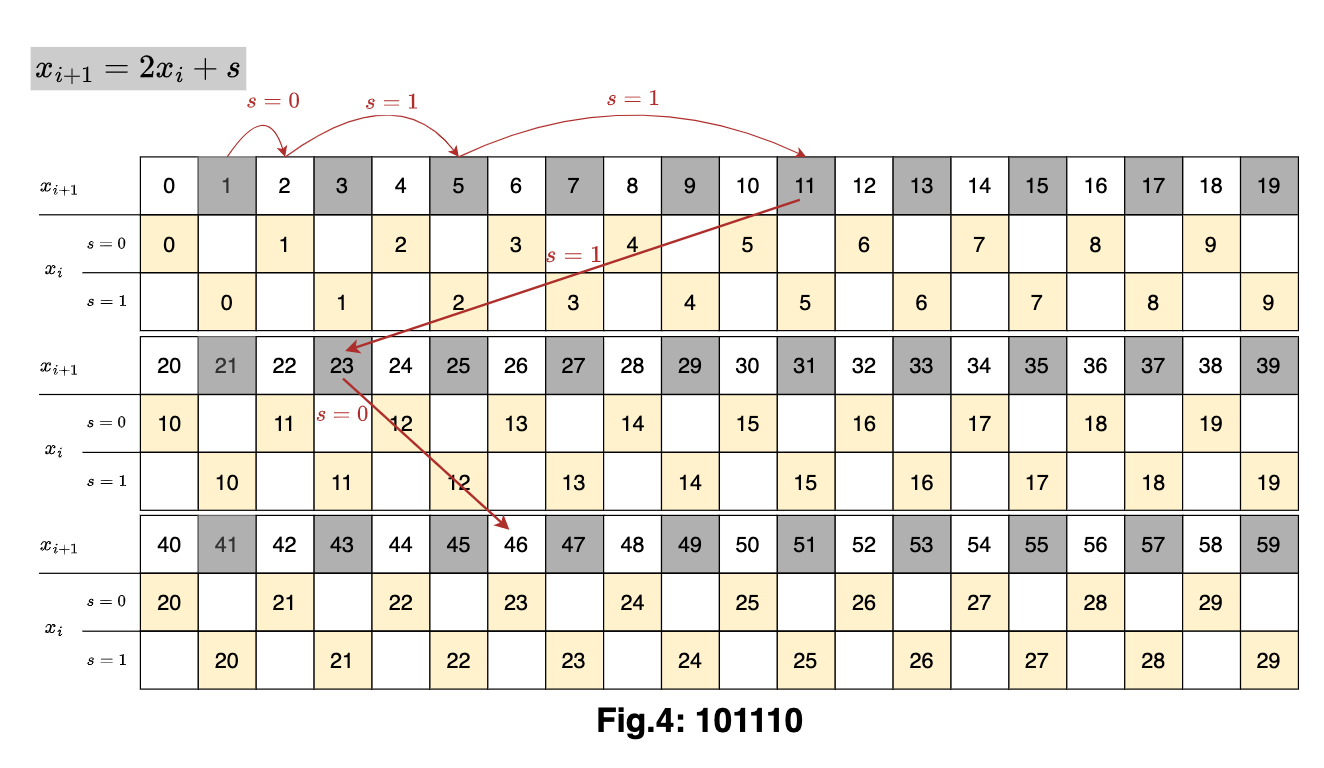
\includegraphics[width=0.89\textwidth]{../24ws_ANS.assets/fig4_0.png}
        \end{center}
    \end{frame}
    \begin{frame}[fragile]{Exa.3: $Pr(0)=1/4, Pr(1)=3/4$}
        \begin{itemize}
            \item<1-> How to encode 101110? 
            \item<2-> What is the encoding function $\mathit{C(s,x_i)}$? $\mathit{x_{i+1} = C(s,x_i) \textcolor{red}{\approx} x_i/p_s}$
            \item<3-> How can we find \textcolor{orange}{the $\mathit{x_i}$ -th appearance of symbol $\mathit{s}$} ?
            \item<4-> 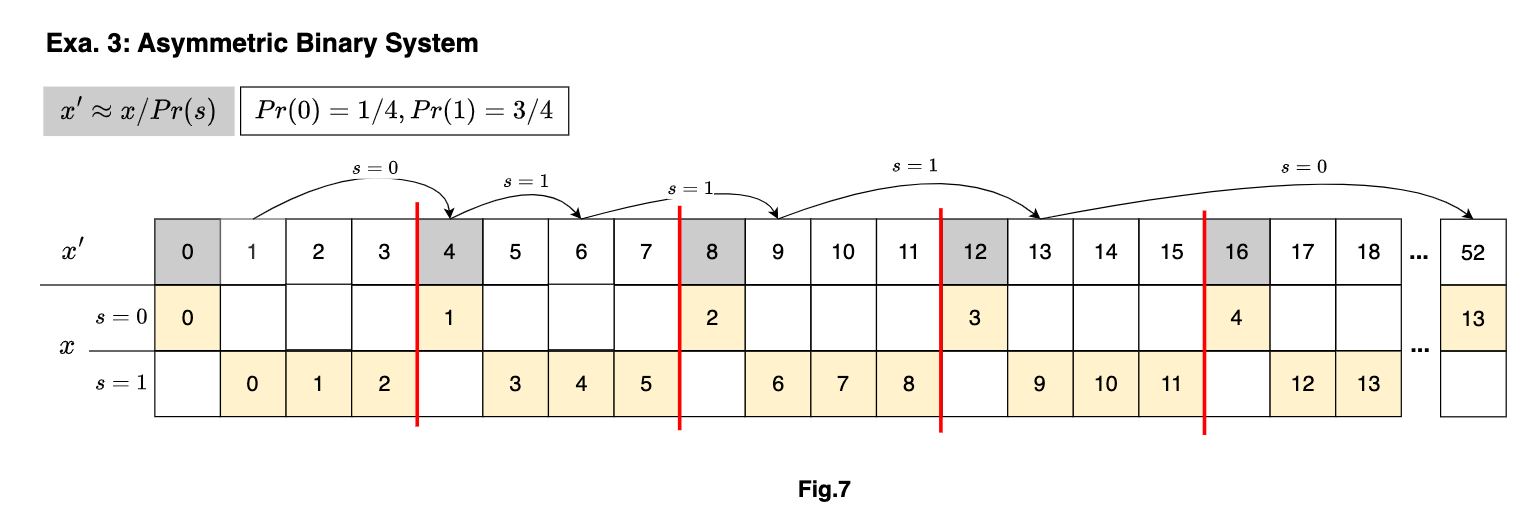
\includegraphics[width=0.8\textwidth]{../24ws_ANS.assets/fig7.png}
        \end{itemize}
    \end{frame}
    
\subsection{Notations}
    \begin{frame}[fragile]{Some Notations}
        \begin{itemize}
            \item<1-> $\mathcal{A} = \{\mathit{s_1, s_2, \dots, s_k}\}$ is the alphabet set
            \item<2-> $\mathit{s}$ is the symbol, if it is used in subscript: $\mathit{s}$ is the current symbol, $\mathit{s}-1$ is the previous symbol,  $\mathit{s}+1$ is the next symbol
            \item<3-> $\mathit{F_s}$ is the absolute frequency of symbol $\mathit{s}$
            \item<4-> $\mathit{m = \sum_{s \in \mathcal{A}} F_s}$ is the total frequency
            \item<5-> $\mathit{c_s = \sum_{s \in \mathcal{A}} F_{s-1}}$ is the cumulative frequency ($\mathit{c_{s+1}}$ is the cumulative frequency of the next symbol)
            \item<6-> $\mathit{p_s = F_s / m}$ is the probability of symbol $\mathit{s}$
            \item<7-> $\mathit{x_i}$ is the current state (next state: $\mathit{x_{i+1}}$, previous state: $\mathit{x_{i-1}}$)
        \end{itemize}
    \end{frame}

\subsection{Encoding Function}
    \begin{frame}[plain]
        \begin{figure}
            \centering
            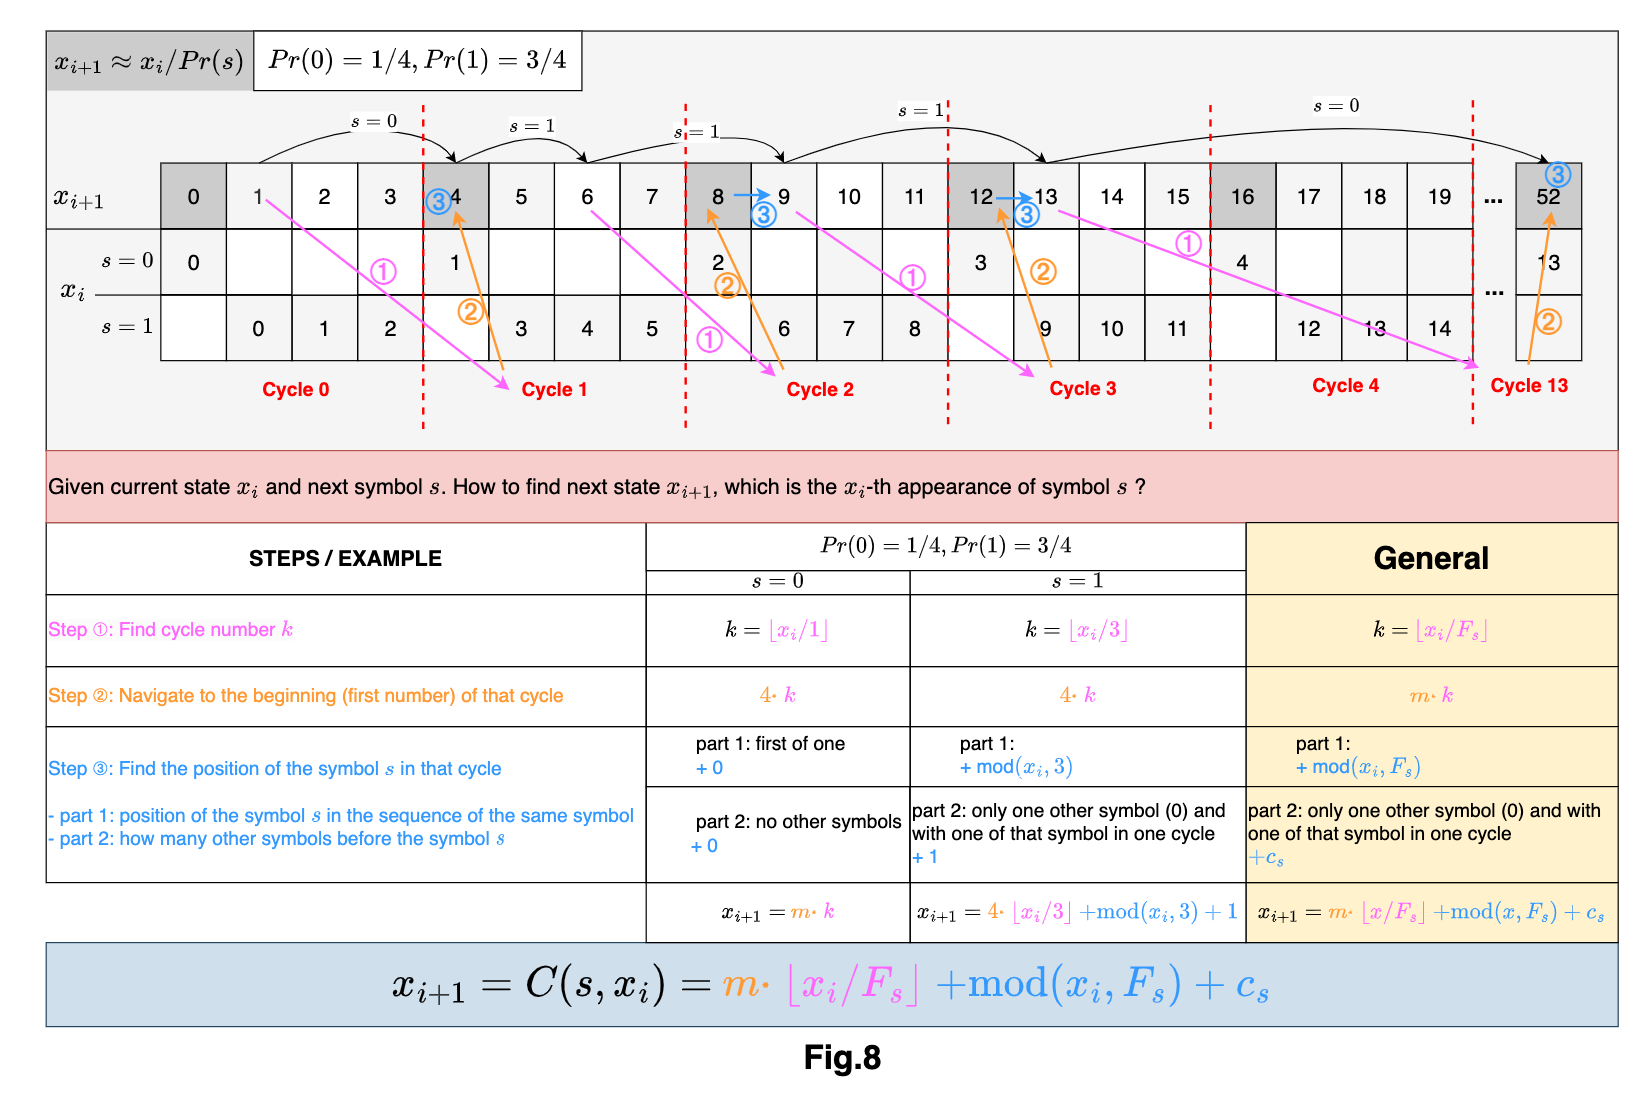
\includegraphics[width=1\textwidth,height=1.07\textheight,keepaspectratio]{../24ws_ANS.assets/fig8.png}
        \end{figure}
    \end{frame}
    \begin{frame}[fragile]{}
        \textbf{Encoding Function \refer{3} \refer{5}:}
        $$ \mathit{x_{i+1} = m \cdot \lfloor x_i/F_s \rfloor + \operatorname{mod}(x_i, F_s) + c_s} $$
        \textit{*$\mathit{m} \cdot $ can be replaced by bit-shifts $<<$, so multiplication is not necessary, it fastens the encoding process}
    \end{frame}
\subsection{Implementation of Encoder}
    \begin{frame}[fragile]{}
        \href{http://localhost:8050}{implementation with python} (\href{https://github.com/hurryclear/cs_theory/tree/data_compression/24ws_data_compression/implementation}{dash app})
        \begin{minted}[fontsize=\scriptsize, linenos, breaklines]{python}
            def rANS_encoder(symbol_counts, s_input):
                cumul_freq = [] # c_s
                sum_freq = 0 # m
                x = 0 # initial state
                output = [] # list to store encoded (symbols, state)
                for count in symbol_counts:
                    cumul_freq.append(sum_freq)
                    sum_freq += count

                for s in s_input:
                    F_s = symbol_counts[s]
                    c_s = cumul_freq[s]
                    x = sum_freq * (x // F_s) + (x % F_s) + c_s
                    output.append((s, x))
                
                L_avg = math.ceil(math.log(x) / math.log(2.0)) / len(s_input)
                return output, x, L_avg, entropy(symbol_counts)
        \end{minted}
    \end{frame}

\subsection{Decoding Function}
    \begin{frame}[plain]
        \begin{figure}
            \centering
            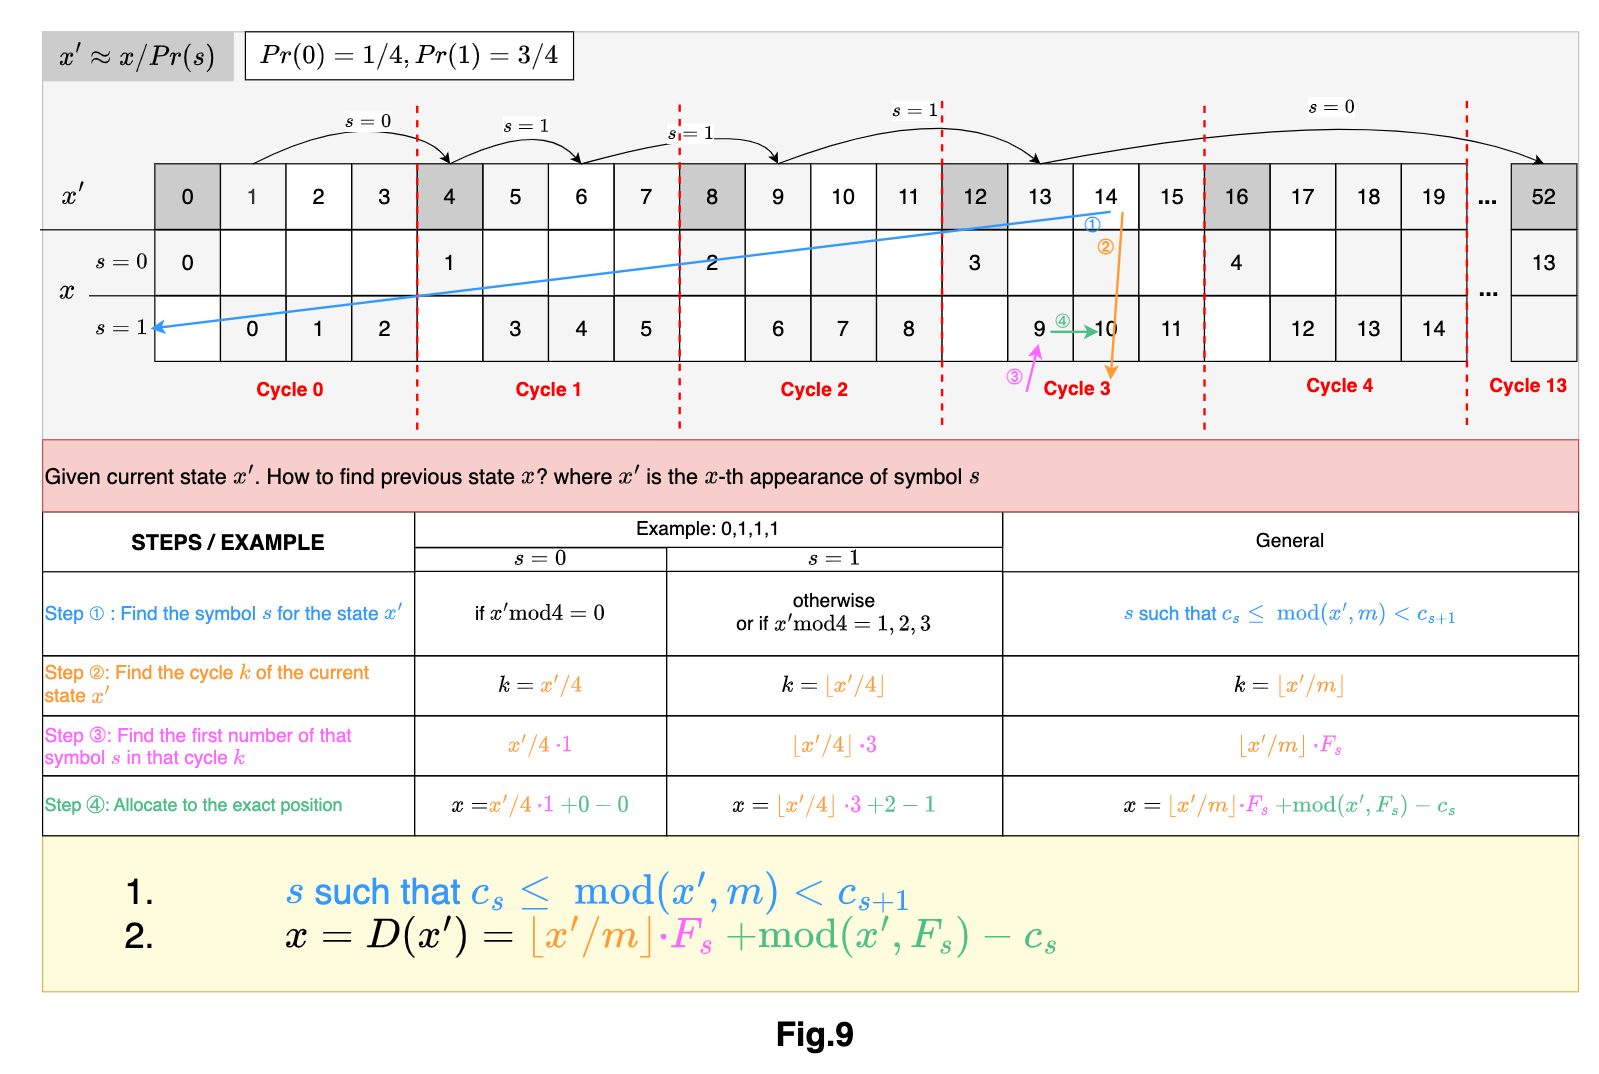
\includegraphics[width=1\textwidth,height=1.07\textheight,keepaspectratio]{../24ws_ANS.assets/fig9.png}
        \end{figure}
    \end{frame}
    
    \begin{frame}[fragile]{}
        \textbf{Decoding Function \refer{3} \refer{5}:}
        \begin{itemize}
            \item $\mathit{s}$ $$ \mathit{s \text{ such that} c_s \leq \text{ mod} (x_i, m) < c_{s+1}} $$
            \item $\mathit{x_{i-1}}$ $$ \mathit{ x_{i-1} = D(x_i)= \lfloor x_i/m \rfloor \cdot F_s + \text{mod}(x_i, F_s) - c_s} $$
        \end{itemize}
        \textit{*$\mathit{x_{i-1}}$ can be replaced by bit-shifts $>>$, so division is not necessary, it fastens the decoding process \\ *mod$\mathit{(x_i, F_s)}$ can be replaced by bitwise AND operation($\& mask$), so mod operation is not necessary}
    \end{frame}
    
\subsection{Implemenation of Decoder}
    \begin{frame}[fragile]{}
        \href{http://localhost:8050}{implementation with python} (\href{https://github.com/hurryclear/cs_theory/tree/data_compression/24ws_data_compression/implementation}{dash app})
        \begin{minted}[fontsize=\scriptsize, linenos, breaklines]{python}
            def rANS_decoder(symbol_counts, x):
                cumul_freq = []  # c_s
                sum_freq = 0 # m
                output = []  # List to store decoded symbols and states
                # compute m and c_s
                for count in symbol_counts:
                    cumul_freq.append(sum_freq)
                    sum_freq += count
                while x > 0:
                    slot = x % sum_freq  # Find the slot in the cumulative frequency range
                    s = bisect_right(cumul_freq, slot) - 1 # Binary search to find the symbol s (slot).
                    F_s = symbol_counts[s]         # Frequency of the symbol
                    c_s = cumul_freq[s]            # Cumulative count of the symbol
                    output.append((s,x))           # Append decoded symbol to the output
                    x = (x // sum_freq) * F_s + x % sum_freq - c_s  # Update the state
                return output, state
        \end{minted}
    \end{frame}
